\subsection{Statistical Study of CTLE Literature}
A survey of prior art published between 2012 and 2025 identifies 16 distinct CTLE architectures reported across major IEEE venues.

\begin{figure}[H]
    \centering
    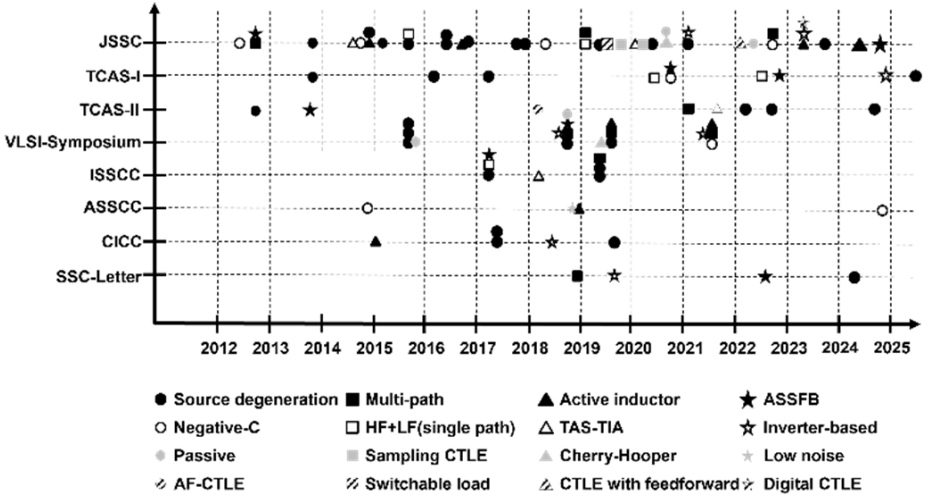
\includegraphics[width=0.8\textwidth]{img/CTLE_img/survey.png}
    \caption{CTLE publications by venue and year (2012-2025)}
    \label{fig:survey_timeline}
\end{figure}

\begin{figure}[H]
    \centering
    \begin{minipage}{0.53\textwidth}
        \centering
        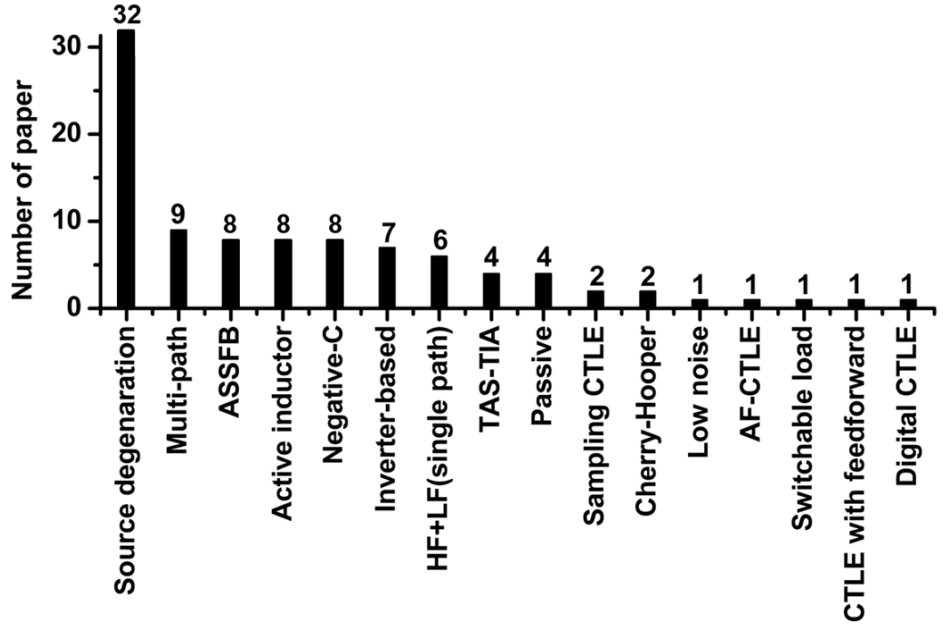
\includegraphics[width=\textwidth]{img/CTLE_img/survey_2.png}
        \captionof{figure}{16 CTLE architectures found in literature survey}
        \label{fig:ctle_architectures}
    \end{minipage}
    \hfill
    \begin{minipage}{0.35\textwidth}
        \centering
        \begin{tabular}{|l|c|}
        \hline
        \textbf{Architecture} & \textbf{Papers} \\ \hline
        Source-Degeneration (SD) & 32 \\ \hline
        Multi-path & 9 \\ \hline
        Active Inductor & 8 \\ \hline
        ASSFB & 8 \\ \hline
        Negative-Capacitance & 8 \\ \hline
        Other Architectures & 18 \\ \hline
        \textbf{Total} & \textbf{83} \\ \hline
        \end{tabular}
        \captionof{table}{Most prevalent CTLE architectures}
        \label{tab:topology_prevalence}
    \end{minipage}
\end{figure}

 The timeline shows the evolution of CTLE designs over this period. The survey reveals that while numerous CTLE architectures exist, only five represent the majority of published designs. The next section focuses on analyzing these five most prevalent architectures along with the passive CTLE:

1. Source-Degeneration CTLE \\
2. Multi-path CTLE  \\
3. Passive \& Active Inductor CTLE \\ 
4. ASSFB CTLE \\ 
5. Negative-Capacitance CTLE \\
6. Passive CTLE\\